% Figure 1 for Paper 01 (The Law of Graphic Equalisation).
%
% The central dynamical structure, drawn: present structure determines
% admissible possibility; collapse realises exactly one continuation; the
% realised successor becomes the antecedent of the next step; whatever the
% realised successor did not absorb is residual.
%
% Standalone: pdflatex fig01_collapse_dynamic.tex
% In-paper  : \input{figures/fig01_collapse_dynamic-body} (see body file)
\documentclass[border=6pt,tikz]{standalone}
\usepackage{amsmath,amssymb,lmodern}
\usetikzlibrary{arrows.meta,positioning,calc,fit,backgrounds}
\newcommand{\Poss}{\mathcal{P}}
\newcommand{\Coll}{\mathcal{C}}
\begin{document}
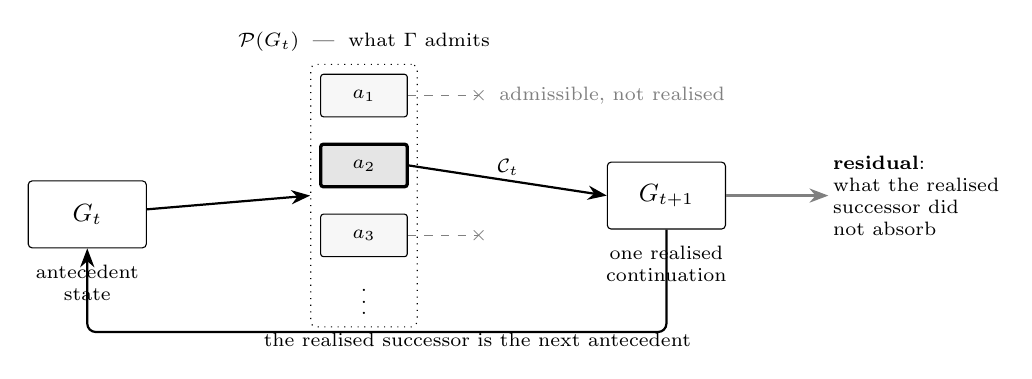
\begin{tikzpicture}[
  >={Stealth[length=2.4mm]},
  node distance=9mm,
  gnode/.style={draw, rounded corners=1.4pt, minimum width=15mm,
                minimum height=8.5mm, font=\small, inner sep=2pt},
  cand/.style={draw, rounded corners=1pt, minimum width=11mm,
               minimum height=5.4mm, font=\scriptsize, inner sep=1pt,
               fill=black!3},
  chosen/.style={cand, very thick, fill=black!10},
  lbl/.style={font=\scriptsize, inner sep=1.5pt},
  flow/.style={->, thick},
  unreal/.style={-, gray, dashed, semithick},
  xmark/.style={inner sep=0pt, font=\scriptsize, gray,
                label={[gray, font=\scriptsize, inner sep=1pt]center:$\times$}},
]
% --- antecedent -------------------------------------------------------
\node[gnode] (gt) {$G_t$};
\node[lbl, below=1.5mm of gt, align=center]
  {antecedent\\state};

% --- the admissible possibility set -----------------------------------
\node[cand] (a1) [above right=8mm and 22mm of gt] {$a_1$};
\node[chosen] (a2) [below=3.2mm of a1] {$a_2$};
\node[cand] (a3) [below=3.2mm of a2] {$a_3$};
\node[cand, draw=none, fill=none] (adots) [below=1.6mm of a3] {$\vdots$};

\begin{scope}[on background layer]
  \node[draw, dotted, rounded corners=2pt, fit=(a1)(a3)(adots),
        inner sep=3.4pt] (pbox) {};
\end{scope}
\node[lbl, above=1mm of pbox] {$\Poss(G_t)$ \;---\; what $\Gamma$ admits};

\draw[flow] (gt) -- node[lbl, above, sloped] {} (pbox.west);

% --- collapse ---------------------------------------------------------
\node[gnode] (gt1) [right=24mm of pbox] {$G_{t+1}$};
\node[lbl, below=1.5mm of gt1, align=center]
  {one realised\\continuation};

\draw[flow] (a2.east) -- node[lbl, above] {$\Coll_t$} (gt1.west);
% admissible but not realised: they stop, they do not contribute
\draw[unreal] (a1.east) -- ++(9mm,0) node[xmark] {};
\draw[unreal] (a3.east) -- ++(9mm,0) node[xmark] {};
\node[lbl, gray, right=1mm of a1, xshift=10mm, anchor=west]
  {admissible, not realised};

% --- the antecedent-state principle -----------------------------------
\draw[flow, rounded corners=3pt]
  (gt1.south) -- ++(0,-13mm) -| (gt.south);
\node[lbl, below=12.5mm of gt1, xshift=-24mm]
  {the realised successor is the next antecedent};

% --- residual ---------------------------------------------------------
\node[lbl, right=13mm of gt1, align=left, anchor=west] (res)
  {\textbf{residual}:\\what the realised\\successor did\\not absorb};
\draw[flow, gray] (gt1.east) -- (res.west);
\end{tikzpicture}

\end{document}
